% !TEX TS-program = xelatex

\documentclass[10pt]{report} 
%\documentclass[9pt]{extreport} 
\usepackage{amssymb}
\usepackage{fontspec}
\setmainfont{Arial}
\usepackage{fullpage}    
\usepackage{graphicx}
%\usepackage{color}
%\usepackage{amsmath}

%\usepackage{mathtools}
\usepackage[top=25mm,bottom=25mm,left=25mm,right=25mm]{geometry}    
\usepackage{a4}            % See geometry.pdf to learn the layout options. There are lots.
\geometry{a4paper} 
\usepackage{graphicx}
\usepackage{wrapfig}
\usepackage{caption}
%\usepackage{float}
\usepackage{setspace}
\usepackage{booktabs}
\usepackage{applekeys}
\usepackage{enumerate} 
\usepackage{enumitem}



%\usepackage{natbib}
%\bibliographystyle{plainnat}

\graphicspath{ {./img/} }

\title{\LARGE Felix Design Guide 2013-14}

\author{Joseph Letts, Felix Editor 2013-14}

\makeatletter
\renewcommand{\@dotsep}{10000} 
\makeatother

%\renewcommand{\contentsname}{Agenda}
\renewcommand{\arraystretch}{1.7}

\DeclareGraphicsExtensions{.pdf,.png,.jpg}
 \begin{document}
\maketitle
\doublespacing
%\titlepage
\pagenumbering{gobble}
\tableofcontents
\singlespacing
%\addtocontents{toc}{\protect\thispagestyle{empty}}
\cleardoublepage %start new page
% \setcounter{page}{1}


\chapter{Introduction}
 The purpose of the Felix Design Guide is to provide a guide for Section Editors to follow while designing their pages for the paper. This should be put together by the Editor-in-Chief each year.
The Design Guide (DG) will explain the styles associated with different elements of the paper and how they should be used to complete the design for each page. If you have any questions, consult the Editor-in-Chief who should be able to give you the best solution for the problem. 

\chapter{Fonts}

Felix (2013-14) uses several font families, so how do you know what to use and when?

\section{Futura}

Futura is the paper's main sans-serif font, used for headlines and general titles. 

\begin{description}
	\item[Futura Bold] The bold weight is used for section titles, article headlines, drop caps, box titles and pull quotes.
	\item[Futura BoldCondensed] The condensed version of the bold weight should be rarely used. It is mainly used for news headlines to give contrast (especially in 'all caps').
	\item[Futura Medium] The medium weight is used for sub-headlines and in-article titles. 
\end{description}

\section{Warnock Pro}

Warnock Pro is the font family used for copy (article text). This is a serif font and is only used in main text (i.e. not headlines/title).

\begin{description}
	\item[Warnock Pro Regular] The regular weight is used for the bulk of the article text
	\item[Warnock Pro Bold] The bold weight is used for emphasis in articles, to highlight interview questions or to draw attention to an informative last paragraph (i.e. event/campaign information)
	\item[Warnock Pro Italic] The italic weight is used to show artist/event names, long stretches of quotations and de-emphasise intro text before an article.
\end{description}

\section{Jigsaw}
 Jigsaw is a font family that has been slightly carried over from the previous design. Generally not used.



\chapter{Images}

Images are a key part of making the page look more appealing to the reader, however they need to be chosen and placed with some consideration.

\section{Image Placement}

Images should only ever be unit column widths in size, i.e. one/two/three/four/five column widths in size. They should never be extended into the next column, since the word wrapped text in the half column they will occupy will tend to be disjointed and may need hypenation.

The only time an image should extend by a half column is if it is contained in a column that is 1.5 times wider than than the usual column width. 

\section{Image Quality}

When sourcing images to use for a page, an editor should look for large images only. If searching via Google Images online, make sure to filter the image search to large images only. After placing the image on your page, check the \textbf{Links panel} in the palette on the right hand side of the screen (also available by using \shiftkey \cmdkey D).

All images should have an \textbf{Effective PPI} of at least \textbf{150} in the links panel.


\section{Image Colour Space}

\begin{wrapfigure}{r}{5cm}
\vspace{-22pt}
\begin{center}
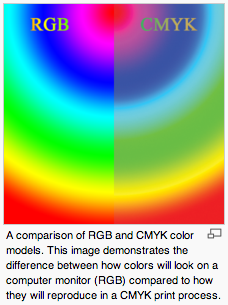
\includegraphics[width=4.8cm]{rgb-cmyk}
\end{center}
\vspace{-50pt}
\end{wrapfigure} 
All images you will encounter on the internet and from a camera will be recorded using the RGB (Red Green Blue), colour space, however printers print using the Cyan Magenta Yellow blacK (CMYK) colour space. This means that we need to convert all of our images into CMYK before we send the paper to the printers. This means that if any images are not easily reproduced in the CMYK colour space (i.e. pictures with large amounts of R, G or B), they can be adjusted before being sent of to print. This can be done using the Felix Droplet (ask Editor for more information).

Please note: Greyscale images do not need to be converted to CMYK, however it is good practise (in order to keep up the habit).

\section{Credits and Captions}


\subsection{Credits}

All images need to be credited. Google Images is not a suitable credit for any image. At the very least, if an image can only be traced back to a blog, the name of the blog can be used as the credit.
Images are credited using the "Photo Credit" paragraph style located in the Felix 2013-14 -> Photo/Image folder in the "Paragraph Styles" panel. Image credits are always placed on the line directly under the image on the right hand side. In some cases when this is not possible the credit can instead be printed in \textbf{white/paper} on a black bar at the bottom of the image.

N.B. When crediting websites, the "https://www" is always omitted. 

\subsection{Captions}

Captions also exist on the line directly under an image. These are left-aligned (never justified) and can fill the space under the picture (up to the credit location). Captions are optional, but credits are mandatory.



\appendix
\chapter{Paragraph Styles}

\begin{tabular}{p{3cm} p{3cm} p{6cm} c } 

Paragraph Style & Font Family & Weight(s) & Size(s) [pt] \\ \hline
Headline  & Futura & Bold & \\
Subheadline & Futura & Medium, Bold & \\
Main Text & Warnock Pro & Regular, Bold, Italic & 9 \\
Photo Caption & Futura & Medium & 9 \\
Photo Credit & Futura & Medium (All Caps) & 6 \\


\end{tabular}









 


% \input{move}

% \input{conclusion}

%\printbibliography
%\bibliography{bibliography}
\end{document}
